\begin{figure*}[t]
  \centering
  \begin{minipage}{0.318\textwidth}
    \centering
    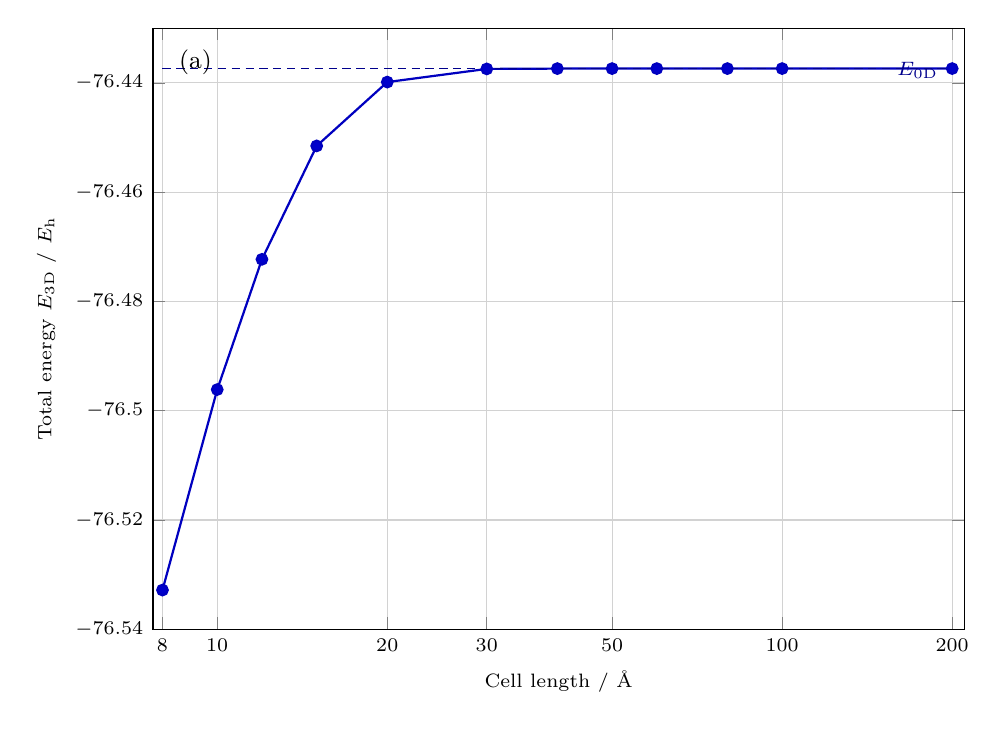
\begin{tikzpicture}
      \begin{axis}[
        width=0.98\linewidth,
        height=0.76\linewidth,
        xmode=log,
        log basis x=10,
        xlabel={Cell length / \AA},
        ylabel={Total energy $E_{\mathrm{3D}}$ / $E_\mathrm{h}$},
        xmin=7.7,
        xmax=210,
        ymin=-76.54,
        ymax=-76.43,
        xtick={8,10,20,30,50,100,200},
        xticklabels={8,10,20,30,50,100,200},
        ytick={-76.54,-76.52,-76.50,-76.48,-76.46,-76.44},
        scaled y ticks=false,
        y tick label style={/pgf/number format/fixed,/pgf/number format/precision=2},
        grid=both,
        minor grid style={gray!18},
        major grid style={gray!35},
        tick label style={font=\scriptsize},
        label style={font=\scriptsize},
      ]
        \addplot+[blue!75!black, thick, mark=*, mark size=1.9pt]
          coordinates {
            (8,-76.53281894254921)
            (10,-76.49612779497798)
            (12,-76.47229243885772)
            (15,-76.45153916705496)
            (20,-76.43985589661881)
            (30,-76.43744818779650)
            (40,-76.43738940213733)
            (50,-76.43738670717899)
            (60,-76.43738601862653)
            (80,-76.43738549312393)
            (100,-76.43738530537355)
            (200,-76.43738513450192)
          };
        \addplot+[blue!55!black, densely dashed, thin, mark=none, domain=8:200]
          {-76.437385109217445};
        \node[anchor=south east,font=\scriptsize,blue!55!black]
          at (rel axis cs:0.98,0.90) {$E_{\mathrm{0D}}$};
        \node[anchor=north west,font=\small] at (rel axis cs:0.02,0.98) {(a)};
      \end{axis}
    \end{tikzpicture}
  \end{minipage}\hfill
  \begin{minipage}{0.318\textwidth}
    \centering
    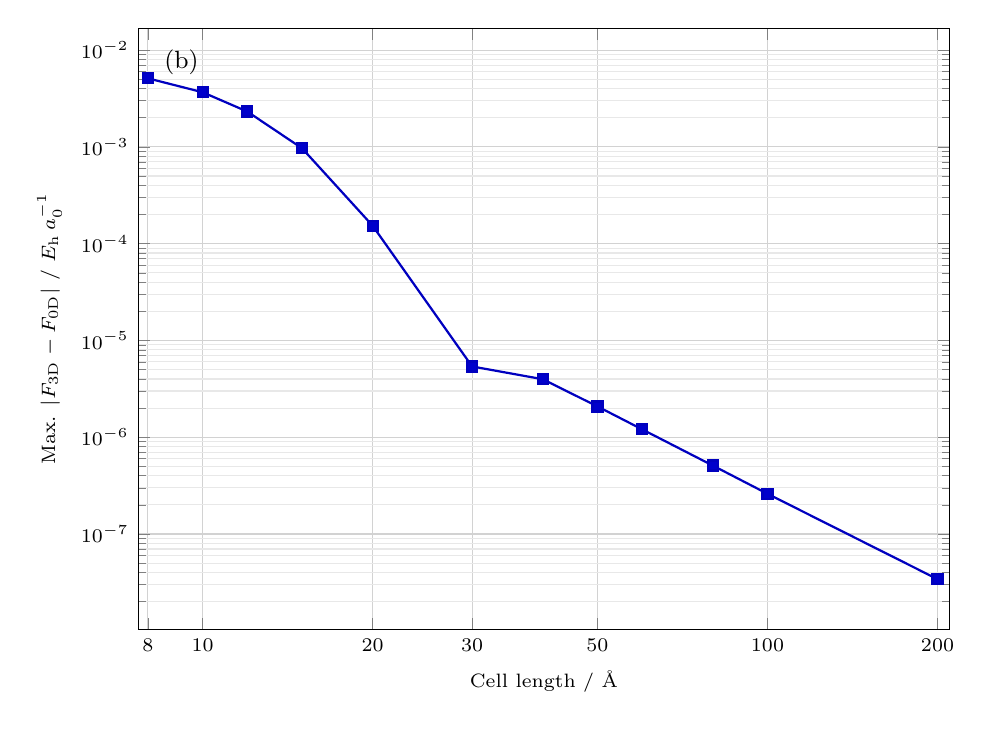
\begin{tikzpicture}
      \begin{axis}[
        width=0.98\linewidth,
        height=0.76\linewidth,
        xmode=log,
        ymode=log,
        log basis x=10,
        log basis y=10,
        xlabel={Cell length / \AA},
        ylabel={Max. $|F_{\mathrm{3D}}-F_{\mathrm{0D}}|$ / $E_\mathrm{h}\,a_0^{-1}$},
        xmin=7.7,
        xmax=210,
        xtick={8,10,20,30,50,100,200},
        xticklabels={8,10,20,30,50,100,200},
        grid=both,
        minor grid style={gray!18},
        major grid style={gray!35},
        tick label style={font=\scriptsize},
        label style={font=\scriptsize},
      ]
        \addplot+[blue!75!black, thick, mark=square*, mark size=1.8pt]
          coordinates {
            (8,0.0051117107)
            (10,0.0036713449)
            (12,0.0023167801)
            (15,0.0009674247)
            (20,0.0001532398)
            (30,0.0000053846)
            (40,0.0000039755)
            (50,0.0000020804)
            (60,0.0000012048)
            (80,0.0000005096)
            (100,0.0000002602)
            (200,0.0000000341)
          };
        \node[anchor=north west,font=\small] at (rel axis cs:0.02,0.98) {(b)};
      \end{axis}
    \end{tikzpicture}
  \end{minipage}\hfill
  \begin{minipage}{0.318\textwidth}
    \centering
    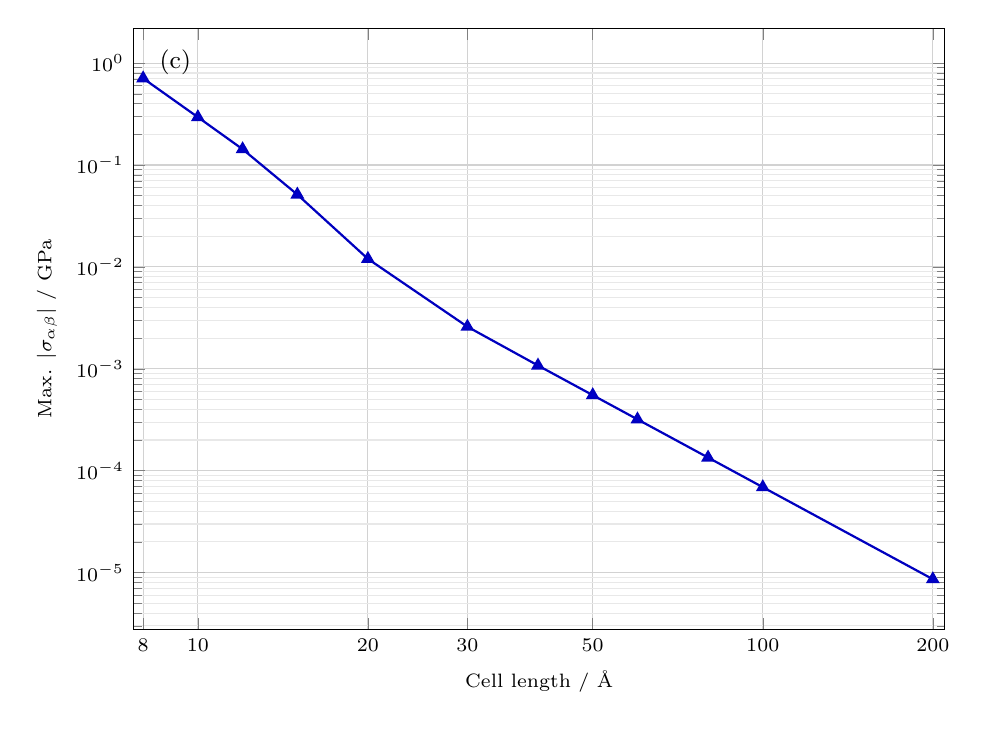
\begin{tikzpicture}
      \begin{axis}[
        width=0.98\linewidth,
        height=0.76\linewidth,
        xmode=log,
        ymode=log,
        log basis x=10,
        log basis y=10,
        xlabel={Cell length / \AA},
        ylabel={Max. $|\sigma_{\alpha\beta}|$ / GPa},
        xmin=7.7,
        xmax=210,
        xtick={8,10,20,30,50,100,200},
        xticklabels={8,10,20,30,50,100,200},
        grid=both,
        minor grid style={gray!18},
        major grid style={gray!35},
        tick label style={font=\scriptsize},
        label style={font=\scriptsize},
      ]
        \addplot+[blue!75!black, thick, mark=triangle*, mark size=2.1pt]
          coordinates {
            (8,0.709263905)
            (10,0.294713793)
            (12,0.142946798)
            (15,0.051296658)
            (20,0.011996772)
            (30,0.002589107)
            (40,0.001077543)
            (50,0.000551416)
            (60,0.000319085)
            (80,0.000134608)
            (100,0.000068918)
            (200,0.000008615)
          };
        \node[anchor=north west,font=\small] at (rel axis cs:0.02,0.98) {(c)};
      \end{axis}
    \end{tikzpicture}
  \end{minipage}
  \caption{Molecular-limit test for one H$_2$O molecule in cubic cells of
  8--200~\AA.  Panel (a) shows the three-dimensionally periodic total energy
  in $E_\mathrm{h}$; the dashed line is the zero-dimensional total-energy
  reference.  Panel (b) shows the largest Cartesian force-component
  difference between the periodic implicit-Gamma and zero-dimensional
  routes.  Because a
  zero-dimensional calculation has no cell derivative, panel (c) instead
  shows the largest absolute component of the analytical periodic stress
  tensor.  With the zero-dimensional quadrupole--quadrupole contraction made
  consistent with the traceless atomic-quadrupole convention, all three
  quantities converge monotonically and the former force plateau is absent.
  Solid lines guide the eye.}
  \label{fig:h2o_molecular_periodic_limit}
\end{figure*}
